%!TEX root = ../dissertation.tex
\chapter{The project}
\label{cap:one}
\newthought{In the last twenty years}, with the advancement of technology, many Internet-based accommodation reservation systems have been developed, allowing travelers to find a place for the night in a fast and easy way. There are two types of online accommodation booking system\cite{9295937}:
\begin{itemize}
    \item property management system, used mainly by hotel or hotel groups to manage their operations;
    \item vacation rental management system, which is for anyone who wants to offer or book a non-hotel accommodation.
\end{itemize}
The first type can easily manage the guests check-in and the room lock access, and all the problems derived by having physical keys, with a simple front desk. However, in a vacation rental management system, the previous process can be a problem. The features of the existing platforms grant the property listing, booking, and transactions. The most common way to manage the check-in process is passing the physical keys, and that requires the encounter between the guests and the host, or sometimes a paid collaborator. This is particularly time-consuming for both the locator and the lessee, opening to the risks of losing keys, or even worse, such as housebreaking and theft. 
Furthermore, we can identify two more categories in the vacation rental management system, which involve whether the host lives in the rented property or not, which are, respectively, remote hospitality and on-site hospitality\cite{10.1145/2675133.2675274}. While in the latter the check-in management requires little effort because it does not involve distance, with remote hospitality it becomes more complicated. A more common scenario is the first type of hosting, in which a properties owner, which lives in a city, has an unused property on the mountain or near the sea, which is listed on a vacation rental management platform. As a consequence, he must go back and forth in order to manage the rented house.
The most widely used vacation rental management system is Airbnb. This platform counts 6 million active listings worldwide, more than 4 million hosts and it covers more than 220 countries and regions. The reason Airbnb is growing so much inside the market is the ease-of-use of its services. Another reason is that the platform try to instill a sense of trust between the two parts. Platforms operating inside a \textit{sharing economy} \cite{10.1145/3334480.3382900} puts a lot of weight on the power of the reviews. Both hosts and guests are encouraged to leave a review on the platform itself. Airbnb focused a lot on this aspect and the presence of a working review system is part of its success.
Another reason for the popularity of Airbnb is the well-designed rent processes, which are fast, easy to use and secure, for all the actors involved in them. For this reason, they are developing more and more features to smooth the existing processes. Airbnb is, for example, pushing hosts to create smart homes to provide a more easy way to access and manage the property\cite{airbnb-smart}. This new feature is called "self check-in", and it is gradually integrated into the platform. Airbnb outline three alternatives to enable self check-in option.
\begin{itemize}
    \item Lockboxes are the most affordable solution. They are a simple locked storage for physical keys, accessible with temporary codes.
    \item Smart-locks are the object of this analysis, they provide temporary access to the building and they can be used with the vendor mobile application.
    \item Keypads allow guests to access by providing a code, previously generated and delivered by the host. They are often inserted into the smart-lock category.
\end{itemize}
This variety of solutions comes with the differences in cost and features, which can confuse the host. The exponential growth of the market contributes to exacerbate the situation. Many companies are proposing their solution, with different features and as a consequence cost. 

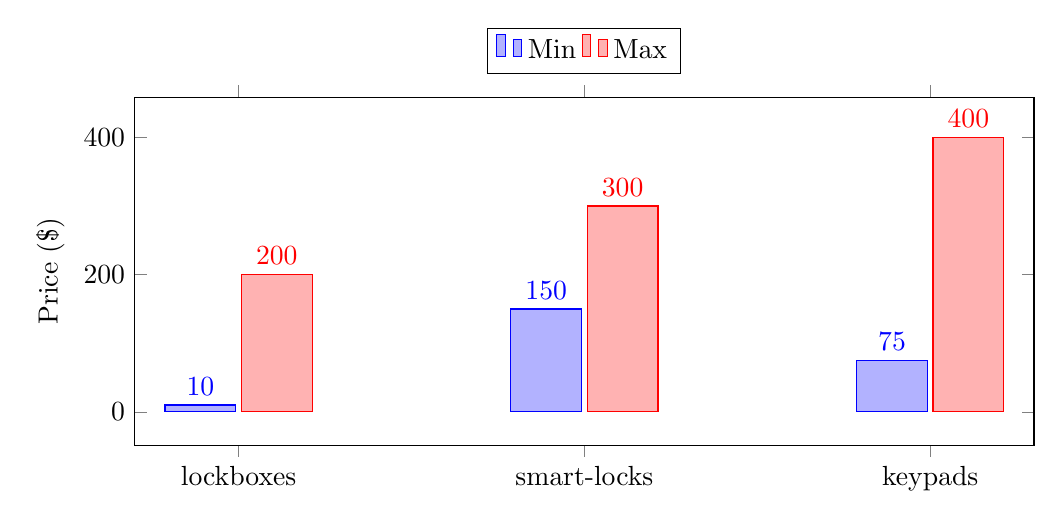
\begin{tikzpicture}
  \begin{axis}[
    enlargelimits=0.15,
    height=6cm,width=13cm,
    bar width=0.9cm,
    legend style={at={(0.5,1.2)},
      anchor=north,legend columns=-1},
    ylabel={Price (\$)},
    symbolic x coords={lockboxes,smart-locks,keypads},
    xtick=data,
    nodes near coords, 
    ybar
    ]
    \addplot coordinates {(lockboxes,10) (smart-locks,150) 
		(keypads,75)};
    \addplot coordinates {(lockboxes,200) (smart-locks,300) 
		(keypads,400)};
    \legend{Min,Max}
  \end{axis}
  \label{graph:lock-price}
\end{tikzpicture}
\\ In the chart \ref{graph:lock-price}, the variations of prices are shown, in relation to the categories identified before.
\\ Lockboxes are the less expensive alternative for a host, but show clear shortcomings. First of all, the use of physical keys is involved, which are exposed to the usual security problems. Moreover, the box must be placed externally, making it vulnerable to any kind of tempering. 
\\ Keypads are not exposed to the lockboxes first problem, because they do not involve keys, but have to be placed externally, making them vulnerable to the public. 
Lastly, most smart locks have wireless interfaces and as such they have the ability to be designed to not expose any hardware to the exterior of the house. Smart-locks have other shortcomings, like the possibility of jamming, the discharge of batteries and the cybersecurity problems of the wireless protocol in use.  
\\ However, despite the price, a smart-lock seems to be the preferred solution for an host, because offers all the features remotely and let the guest feel safer. 
As shown in this investigation \cite{10.1145/3334480.3382900}, in a population of Airbnb hosts in the United States who decide to install smart devices in their rented properties, all of them had installed a smart lock. Their opinion was mostly positive, except for the problems described before. 
\\ A final argument involves the advantage of using smart locks, when managing more than one property. Analyzing the data of the population of Airbnb\cite{airbnbaboutus} is easy to notice that the number of listings is significantly more than the number of hosts. As such, the host having more than one property listed can be approximately be the majority. 
Suppose you are a host with more than one property listed on a vacation rental management system, such as Airbnb, and live far from them, the common way he has to manage their guests is to go to their rented house and meet them in person. If the host decides to install a smart-lock or a keypad, then the problem is solved, but he has to face with another one. The number of solutions is different for each type of door and even the vendor can be different. Moreover, after this type of investment, what an host expects is a sort of automation, from the receiving of the book to the generation of the access permission. 
\\ The solution proposed in this thesis is an portal for host, in which an host can connect all the smart-lock account he owns. This let him to pair the devices, control remotely, generate keys based on the reservation and send that to the guests, without caring about the smart-locks model and provider. The idea is to create a central tool to manage all the properties in one place and give the opportunity of linking all the rental management systems account.